%************************************************
\chapter{User Guide}\label{ch:user_guide}
%************************************************
In this chapter we will walk the system designer through the steps required to set up a simulation from scratch. It also covers how to interact with the environment from the simulation user's point of view. The user guide is written by example, using a concrete environment model -- the childrpoof.blend model which was used in the evaluation). To set up a simulation based on a different model, simply use the other model and take particular configuration actions as required by your use case.

%************************************************
\section{Prerequisites} % (fold)
\label{sec:sd_prerequisites}
%************************************************
To get started, you will need to get your hands on 3 gems:
\begin{enumerate}
	\item The jMonkey Engine 3.0\footnote{\url{http://hub.jmonkeyengine.org/downloads}} development platform, a NetBeans based IDE.
	\item The EgoSim\footnote{\url{https://github.com/ksza/EgoSim/archive/master.zip}} framework from the project's git repository.
	\item The example simulated environment's model\footnote{\url{http://karolyszanto.ro/MastersThesis/evaluation/egosim/media/models/childproof.blend}}.
\end{enumerate}

Unzip the JMonkleyEngine Platform and run it. On the first run you will be asked to configure the working directory. Please do so!\\

From the File menu, select the ''Import Project > From ZIP...'' option. Point to the location of the EgoSim zip you've recently downloaded. This will import the BodyCentricSim project in your workspace.
% section sd_prerequisites (end)
%************************************************
\section{Importing the environment model} % (fold)
\label{sec:sd_import_env_model}
%************************************************
Next, you will import the environment model into the project. Expand the ''Assets/Scene'' folder. Create a new folder, ''Scenes/childproof''. To create a new folder, from the ''File'' menu select the ''New File...'' option. In the dialog, select ''Other'' and ''New Folder'', as depicted in Figure \ref{fig:sd_create_folder}.
\begin{figure}[H]
	\centering
	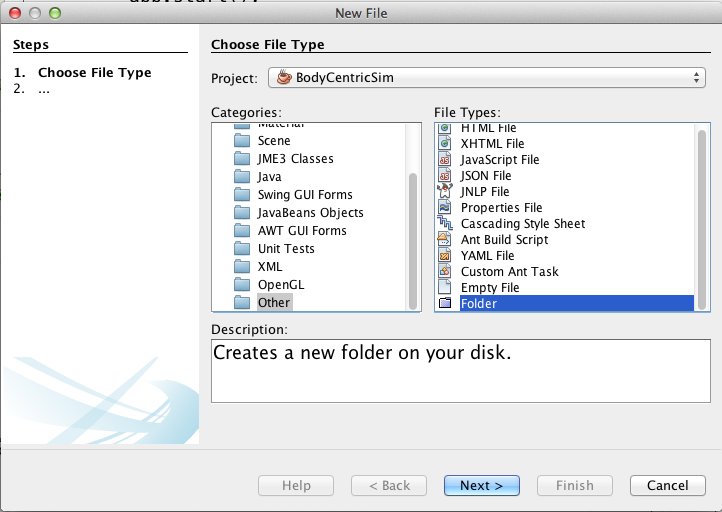
\includegraphics[width=\linewidth]{gfx/Chapter_SD_UserGuide/create_new_folder}
	\caption{Create a new folder within the Scenes folder}
	\label{fig:sd_create_folder}
\end{figure}

Copy the ''childproof.blend'' file into this folder. Once you see the file in the IDE, right click it and ''Convert to j3o Binary''. This convert it to jMonkey format.
% section sd_import_env_model (end)
%************************************************
\section{Setting up the simulation} % (fold)
\label{sec:sd_setup_simulation}
%************************************************
In the ''Source Packages'' folder, under the ''dk.itu.bodysim'' package, create a new class, ChildProofApp. Make this class extend EgocentricApp. In the implementation of the ''createEnvironmentScene'', simply write:
\begin{lstlisting}[caption={Loading a j3o environment},label={lst:importing_model}]
return new GenericEnvironment("Scenes/childproof/childproof.j3o", "ChildProof", assetManager);
\end{lstlisting}

Next, create a main method for your class:
\begin{lstlisting}[caption={Starting the app},label={lst:starting_the_simulation}]
ChildProofApp app = new ChildProofApp(); 
app.start();
\end{lstlisting}

The ChildProofApp class should look similar to:
\begin{lstlisting}[caption={Full class implementation of a new simulation created with EgoSim},label={lst:final_childproof}]
package dk.itu.bodysim;

import com.jme3.scene.Node;
import dk.itu.bodysim.environment.GenericEnvironment;

public class ChildProofApp extends EgocentricApp {

    @Override
    protected Node createEnvironmentScene() {
        return new GenericEnvironment("Scenes/childproof/childproof.j3o", "ChildProof", assetManager);
    }

    public static void main(String[] args) {
        ChildProofApp app = new ChildProofApp();
        app.start();
    }
}
\end{lstlisting}

Now your set! Inside the ChildproofApp hit the SHIFT+F6 key combination. In the settings window just start it up with the default configuration. This will start up the simulation! In here you can control the avatar, move around the environment, NOT walk through walls and objects. The EgoSim took care of this for you.\\

You will notice that you see the environment from a child's perspective: the height of the agent is smaller.\\

At this point, you notice the agent can't interact with any objects. That's because none of them have been augmented with context data! You can notice this by opening, on your second display, the ContextClient\footnote{\url{http://localhost:8182/context/view/set?name=all}} in a browser.
% section sd_setup_simulation (end)
%************************************************
\section{Identifying objects to monitor} % (fold)
\label{sec:sd_identify_objects}
%************************************************
In the assets, right click the ''Scenes/childproof/childproof.j3o'' file and select ''Edit in SceneComposer'' as illustrated in Figure \ref{fig:sd_edit_in_scene_composer}.
\begin{figure}[H]
	\centering
	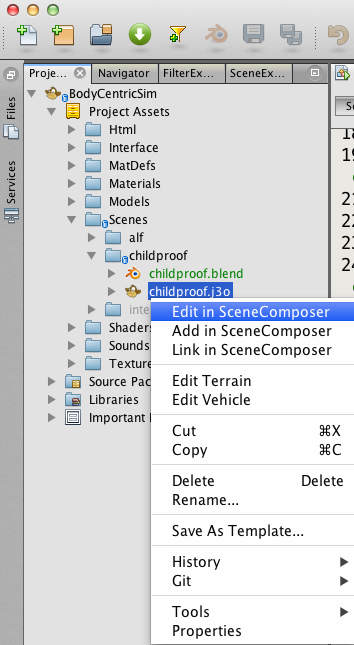
\includegraphics[width=0.5\linewidth]{gfx/Chapter_SD_UserGuide/edit_in_scene_composer}
	\caption{Edit in Scene Composer}
	\label{fig:sd_edit_in_scene_composer}
\end{figure}

To see the environment, you'll have to ''turn on the lights'', as depicted in Figure \ref{fig:sd_light_in_scene_composer}.
\begin{figure}[H]
	\centering
	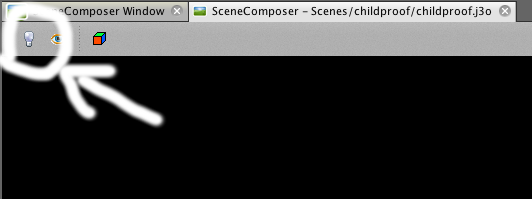
\includegraphics[width=\linewidth]{gfx/Chapter_SD_UserGuide/scenecomposer_light}
	\caption{Turning on the light in Scene Composer}
	\label{fig:sd_light_in_scene_composer}
\end{figure}

Suppose that the objects you want to track in this scenario are the Outlets and all the small objects that might be inserted into them; in this case, the pen on the living room table. These objects are highlighted in the screen-shot from Figure \ref{fig:sd_objects_to_identify}.
\begin{figure}[H]
	\centering
	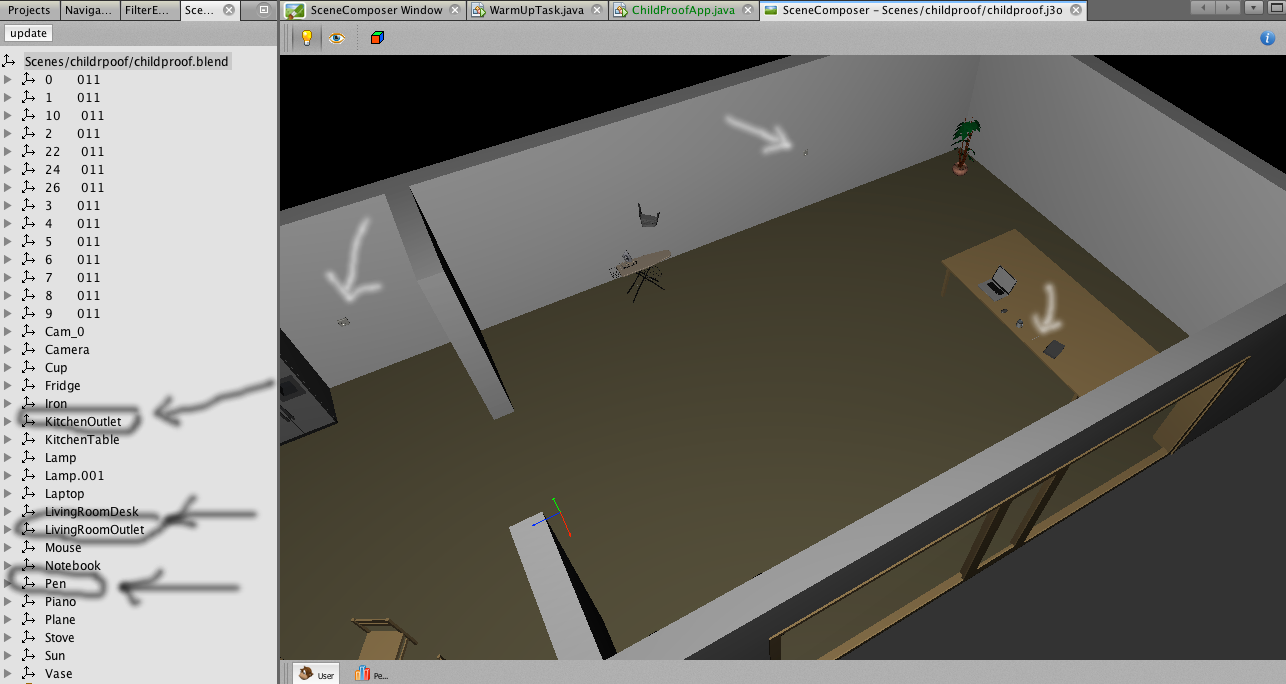
\includegraphics[width=\linewidth]{gfx/Chapter_SD_UserGuide/objects_to_identify}
	\caption{Example objects to identify in the Scene Composer}
	\label{fig:sd_objects_to_identify}
\end{figure}

Identify the objects in the ''SceneExplorer Window'' on the left or by RIGHT-CLICKing on them in the ''SceneComposer''. Either way, as you identify them, they get highlighted in the ''SceneComposer'' on the right, as depicted in Figure \ref{fig:sd_scene_composer}.
\begin{figure}[H]
	\centering
	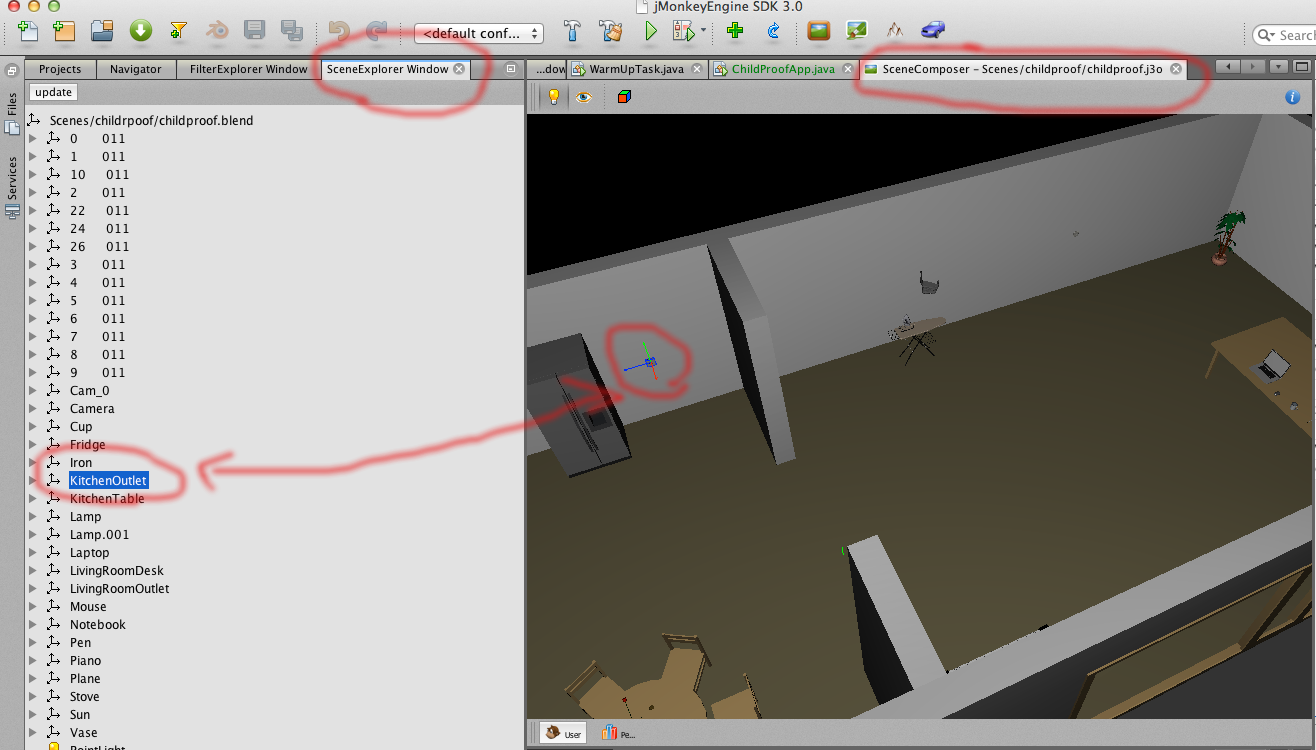
\includegraphics[width=\linewidth]{gfx/Chapter_SD_UserGuide/scenecomposer}
	\caption{Scene Composer}
	\label{fig:sd_scene_composer}
\end{figure}

To augment the objects with context data:
\begin{enumerate}
	\item Right click the object in the ''SceneComposer Window'' and select the ''Add User Data'' as illustrated in Figure \ref{fig:sd_add_user_data}.
		\begin{figure}[H]
			\centering
			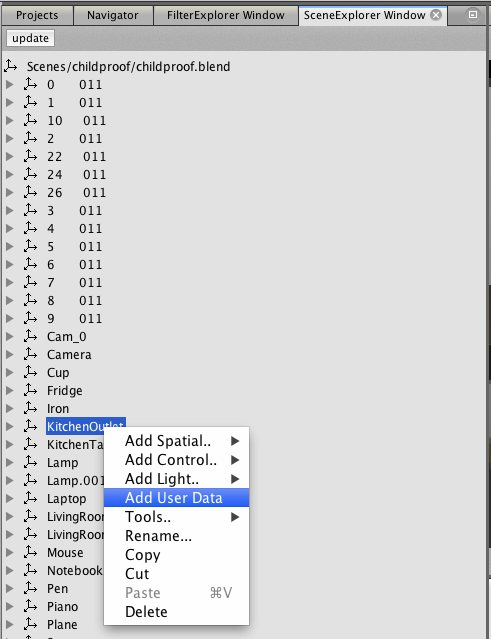
\includegraphics[width=0.8\linewidth]{gfx/Chapter_SD_UserGuide/add_user_data}
			\caption{Add User Data action}
			\label{fig:sd_add_user_data}
		\end{figure}

	\item In the name field enter enter EGOCENTRIC\_CONTEXT\_DATA. From the drop-down select ''Custom'' and choose ''dk.itu.bodysim. context.EgocentricContextData''. This will bring up the configuration form depicted in Figure \ref{fig:sd_config_form}.
		\begin{figure}[H]
			\centering
			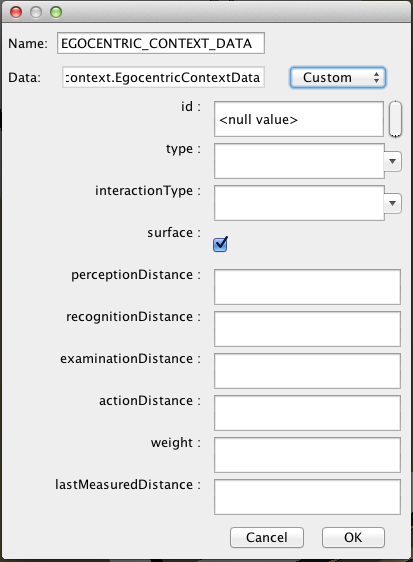
\includegraphics[width=0.8\linewidth]{gfx/Chapter_SD_UserGuide/ssmconfig}
			\caption{Egocentric Context Data Configuration Form}
			\label{fig:sd_config_form}
		\end{figure}

	\item Configure the ID with a unique name (e.g. KitchenOutlet for the outlet in the kitchen) and the ''interactionType'' with ''CUSTOM'' for Outlets (otherwise, the agent will be able to pick it up) and ''PICK\_UP'' for the Pen.

	\item The rest of the parameters will take meaningful default values. Although, to fine tune the classification, the option to configure them is there.

	\item Once done, hit the OK button.
\end{enumerate}

After you have configured all the objects you want to track, from the File menu select the ''Save All'' option.\\

You can close the SceneComposer now.\\
% section sd_identify_objects (end)
%************************************************
\section{Running the simulation} % (fold)
\label{sec:sd_running_the_simulation}
%************************************************
Run the simulation once again. You can notice in the ContextClient\footnote{\url{http://localhost:8182/context/view/set?name=all}} how the objects you've augmented, get classified in the SSM sets.\\

During the simulation, you can also access the API\footnote{\url{http://localhost:8182/context/api/set?name=all}} endpoint which provides the data in JSON format.\\

You can now move around the environment, pick up the Pen and interact with the Outlets.
% section sd_running_the_simulation (end)